\documentclass[12pt]{article}
\usepackage[margin=1in]{geometry}
\usepackage{amsmath, amsthm, amssymb, amsfonts, breqn, graphicx}


\theoremstyle{definition}
\newtheorem{problem}{Problem}
\renewcommand*{\proofname}{Solution}
\newenvironment{custompbm}[1]
  {\renewcommand\theproblem{#1}\problem}
  {\endproblem}
\renewcommand{\theenumi}{\alph{enumi}}


\newcommand{\E}{\text{E}}
\newcommand{\V}{\text{Var}}
\newcommand{\Co}[2]{\text{Cov}({#1}, {#2})}
\newcommand{\pdf}{\text{pdf}}
\newcommand{\pmf}{\text{pmf}}
\newcommand{\me}{\mathrm{e}}
\newcommand*\diff{\mathop{}\!\mathrm{d}}
\newcommand{\vect}[1]{\boldsymbol{#1}}
\newcommand{\mx}[1][t]{\mu_X({#1})}
\newcommand{\gx}[2]{\gamma_X({#1}, {#2})}


\title{Homework Assignment 8}
\author{Matthew Tiger}


\begin{document}


\maketitle


% Problem 2.15
\begin{custompbm}{2.15}
  Suppose that $\{X_t\}$ is a stationary process satisfying the equations
  \[
    X_t = \phi_1 X_{t-1} + \dots + \phi_p X_{t-p} + Z_t,
  \]
  where $\{Z_t\} \sim \text{WN}(0, \sigma^2)$ and $Z_t$ is uncorrelated with
  $X_s$ for each $s<t$. Show that the best linear predictor $P_nX_{n+1}$ of $X_{n+1}$
  in terms of $1, X_1, \dots, X_n$, assuming $n>p$ is
  \[
    P_n X_{n+1} = \phi_1 X_n + \dots + \phi_p X_{n + 1 - p}.
  \]
  What is the mean squared error of $P_nX_{n+1}$?
\end{custompbm}

\begin{proof}
  Note that $\{X_t\}$ is an AR($p$) process and that $P_n X_{n+1} = \phi_1 X_n + \dots + \phi_p X_{n + 1 - p}$
  is the best linear predictor in terms of $1, X_1, \dots, X_n$ if $\vect{a_n} = (\phi_1, \phi_2, \dots, \phi_p, 0, \dots, 0)^{\intercal}$
  is the solution to the Yule-Walker equations $\sum_{i=1}^n \gamma(h-i) a_i = \gamma(h)$
  for $h=1,\dots,n$. Since $\{X_t\}$ is an AR($p$) process, we know that
  $\gamma(h) = \sigma^2 \sum_{j=0}^{\infty} \psi_j \psi_{j+h}$ where $\psi_j = \sum_{k=1}^p \phi_k \psi_{j-k}$
  and $\psi_0 = 1$ for $h > 0$.

  Thus, if $n \geq h \geq p \geq 1$,
  \begin{align*}
    \sum_{i=1}^n \gamma(h-i) a_i &= \sum_{i=1}^p \phi_i \gamma(h-i) \\
    &= \sigma^2 \sum_{i=1}^p \phi_i \sum_{j=0}^\infty \psi_j \psi_{j+h-i} \\
    &= \sigma^2 \sum_{j=0}^\infty \psi_j \sum_{i=1}^p \phi_i \psi_{j+h-i} \\
    &= \sigma^2 \sum_{j=0}^\infty \psi_j \psi_{j+h} = \gamma(h)
  \end{align*}
  since $\sum_{i=1}^p \phi_i \psi_{j+h-i} = \psi_{j+h}$ and the equation holds for $n \geq h \geq p$.

  If $1 \leq h < p < n$,
  \begin{align*}
    \sum_{i=1}^n \gamma(h-i) a_i &= \sum_{i=1}^h \phi_i \gamma(h-i) + \sum_{i=h+1}^p \phi_i \gamma(i-h) \\
    &= \sigma^2 \sum_{i=1}^h \phi_i \sum_{j=0}^\infty \psi_j \psi_{j+h-i} + \sigma^2 \sum_{i=h+1}^p \phi_i \sum_{j=0}^\infty \psi_j \psi_{j+i-h} \\
    &= \sigma^2 \sum_{j=0}^\infty \psi_j \sum_{i=1}^h \phi_i \psi_{j+h-i} + \sigma^2 \sum_{j=0}^\infty \psi_j \sum_{i=h+1}^p \phi_i \psi_{j+i-h}\\
    &= \sigma^2 \sum_{j=0}^\infty \psi_j \left(\sum_{i=1}^h \phi_i \psi_{j+h-i} + \sum_{i=h+1}^p \phi_i \psi_{j+i-h}\right)\\
    &= \sigma^2 \sum_{j=0}^\infty \psi_j \sum_{i=1}^p \phi_i \psi_{j+h-i} \\
    &= \sigma^2 \sum_{j=0}^\infty \psi_j \psi_{j+h} = \gamma(h)
  \end{align*}
  and the equation holds for $1 \leq h < p < n$ showing that $\vect{a_n}$ is
  indeed the best linear predictor of $X_{n+1}$ in terms of $1, X_1, \dots, X_n$.

  The mean squared error of $P_nX_{n+1}$ is given by
  \begin{align*}
    \gamma(0) - \sum_{i=1}^n a_i \gamma(i)
    = \sigma^2\left(\sum_{j=0}^\infty \psi_j^2 - \sum_{j=0}^\infty \psi_j \sum_{i = 1}^p \phi_i \psi_{j+i}\right)
    = \sigma^2\sum_{j=0}^\infty \psi_j \left(\psi_j - \sum_{i = 1}^p \phi_i \psi_{j+i}\right).
  \end{align*}
\end{proof}


\begin{custompbm}{2.16}
  As in the book.
\end{custompbm}

\begin{proof}
  For the \texttt{SUNSPOTS.tsm} data, after fitting an AR(2) model to the mean corrected
  data we obtain the following graphs for the ACF and PACF of the model:

  \vskip 3mm
  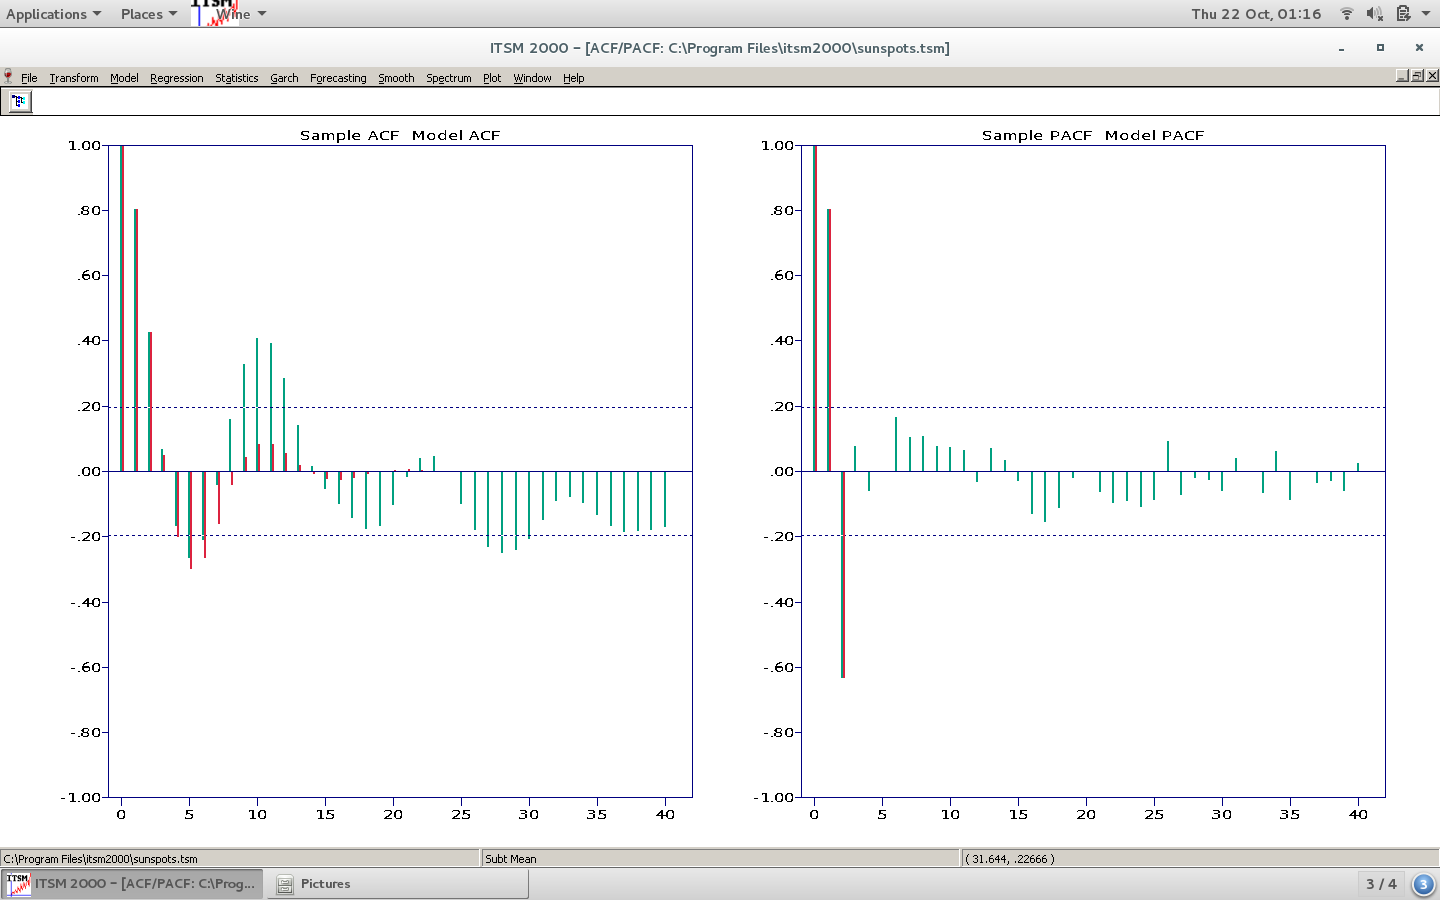
\includegraphics{acf_pacf}

  with parameters $\phi_1 = 1.318$, $\phi_2 = -0.6341$, and $\sigma^2 = 232.895$.
\end{proof}


\begin{custompbm}{2.17}
  As in the book.
\end{custompbm}

\begin{proof}
  Following the instructions presented in the book using the fitted AR(2) model to
  the \texttt{SUNSPOTS.tsm} data in problem 2.16, we have the following predictions
  for lags $t = 101, \dots, 110$:

  \vskip 3mm
  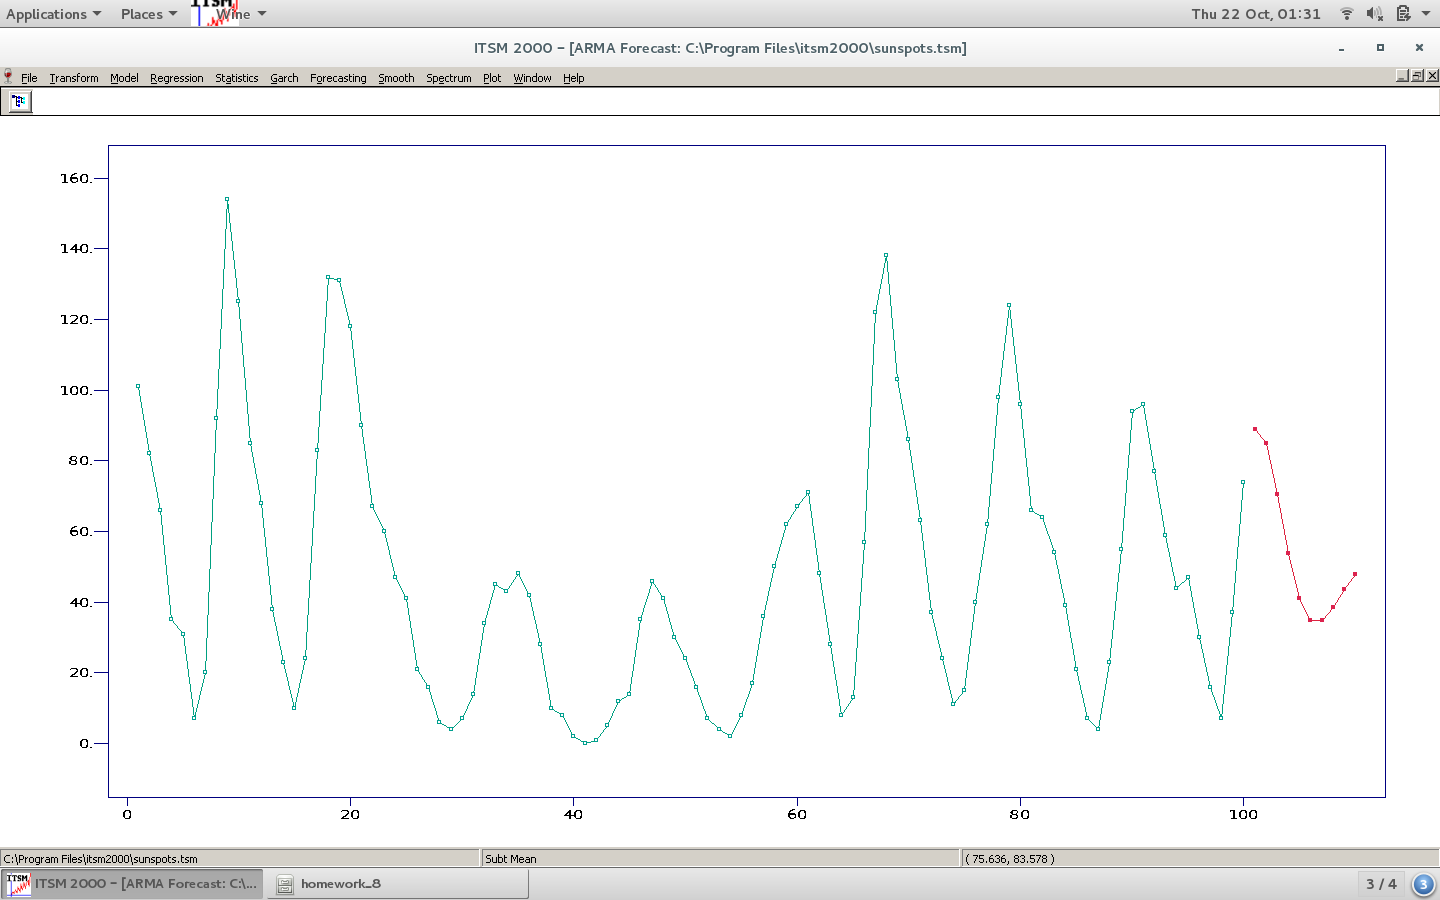
\includegraphics{forecast}
\end{proof}

\end{document}
